

\documentclass{article}
\usepackage[a4paper, total={6in, 8in}]{geometry}

\usepackage{booktabs} % Required for better horizontal rules in tables

\usepackage{array} % Required for manipulating table columns
\usepackage{caption} % Required for customizing captions
\usepackage{enumitem} % Required for list customization
\usepackage{hyperref} % Required for links
\usepackage{graphicx} % Required for including images


\usepackage{tikz}
\usetikzlibrary{shapes,snakes}
\usepackage{amsmath,amssymb}

\usepackage{xcolor}
\PassOptionsToPackage{svgnames}{xcolor}
\usepackage{tcolorbox}
\usepackage{lipsum}
\tcbuselibrary{skins,breakable}
\usetikzlibrary{shadings,shadows}



\definecolor{BgBiblio}{RGB}{255,103,103}
\definecolor{BgTitleBiblio}{RGB}{255,0,0}

\newenvironment{ImportantBiblio}[1]{%
    \tcolorbox[beamer,%
    noparskip,breakable,
    colback=BgBiblio,colframe=BgTitleBiblio,%
    colbacklower=red!75!green,%
    title=#1]}%
    {\endtcolorbox}


\definecolor{BgExp}{RGB}{139,161,255}
\definecolor{BgTitleExp}{RGB}{0,46,255}

\newenvironment{ImportantExp}[1]{%
    \tcolorbox[beamer,%
    noparskip,breakable,
    colback=BgExp,colframe=BgTitleExp,%
    colbacklower=red!75!green,%
    title=#1]}%
    {\endtcolorbox}


\definecolor{BgProtocole}{RGB}{170,170,170}
\definecolor{BgTitleProtocole}{RGB}{55,55,55}


\newenvironment{ProtocoleExp}[1]{%
    \tcolorbox[beamer,%
    noparskip,breakable,
    colback=BgProtocole,colframe=BgTitleProtocole,%
    colbacklower=red!75!green,%
    title=#1]}%
    {\endtcolorbox}


\definecolor{BgEtude}{RGB}{143,255,131}
\definecolor{BgTitleEtude}{RGB}{15,156,0}


\newenvironment{EtudeExp}[1]{%
    \tcolorbox[beamer,%
    noparskip,breakable,
    colback=BgEtude,colframe=BgTitleEtude,%
    colbacklower=red!75!green,%
    title=#1]}%
    {\endtcolorbox}


\title{Journal Calibration} % Article title, use manual lines breaks (\\) to beautify the layout




\begin{document}




\section*{Salle haute-pression}

\subsection*{Calibration octobre 2024}




Il y aura deux positions $x_{Lp2}$ : \begin{itemize}
    \item à 10.00mm pour utiliser l'OPO entre 590 et 650 nm : bonne configuration qui focalise au mieux la source SHG et la source OPO, tout en ayant $\Delta z = 0$.
    \item à 12.00mm pour utilise l'OPO entre 660 et 720 nm : moins bonne focalisation SHG, mais permet $\Delta z = 0$.
\end{itemize}
Les cartes à prendre sont : \begin{itemize}
    \item le 01 Oct : carte de 500 à 590 nm, avec $x_{Lp2} = 10.00$ mm.
    \item Le 04 Oct : carte de 610 à 650 nm, avec $x_{Lp2} = 10.00$ mm.
    \item Le 07 Oct : carte de 520 à 600 nm, avec $x_{Lp2} = 10.00$ mm.
    \item Le 07 Oct : carte de 660 à 720 nm, avec $x_{Lp2} = 12.00$ mm.
    \end{itemize}

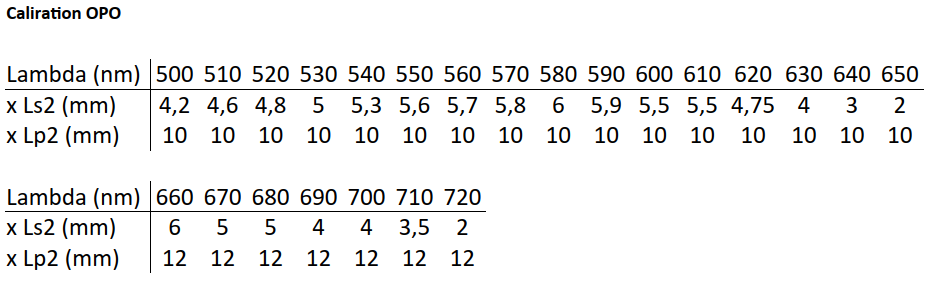
\includegraphics[width=0.9\textwidth]{Figures/calib_salle_haute_pression_octobre_2024.png}





\subsection*{Calibration 05 Novembre 2024}

Entre octobre et novembre 2024, la cavité du Maitai s'est désalignée. On l'a replacée et fixée, et l'OPO a remarché sans avoir besoin d'être réaligné. Cependant, on est pas garanti qu'il a les même propriétés (divergence, taille faisceau) qu'avant. Il faudra donc refaire  une calibration si possible.

Pour bien se repérer, je continue de placer la lentille de sonde dans les positions de référence calibrées. Si beosin, j'ajuste la lentille de pompe pour avoir $\Delta z = 0$.
\end{document}